\documentclass[12pt]{article}
\usepackage{nips11submit_e,times}
%\RequirePackage[OT1]{fontenc}
\RequirePackage{amsbsy,amsmath,amssymb,amsthm}
\RequirePackage{graphicx}

\newcommand{\reals}{\mathbb{R}}
\newcommand{\trans}{\mathrm{T}}
\DeclareMathOperator*{\Tr}{Tr}
\DeclareMathOperator*{\diag}{diag}
\DeclareMathOperator*{\rank}{rank}
\newcommand{\Normal}[1][]{\mathcal{N}_{#1}}
\newcommand{\Wishart}[1][]{\mathcal{W}_{#1}}
\DeclareMathOperator*{\argmin}{argmin}

\newcommand{\prob}{\mathbb{P}}
\newcommand{\E}{\mathbb{E}}
\DeclareMathOperator*{\RSS}{RSS}

\theoremstyle{plain}
\newtheorem{theorem}{Theorem}[section]
\newtheorem{definition}[theorem]{Definition}
\newtheorem{corollary}[theorem]{Corollary}
\newtheorem{lemma}[theorem]{Lemma}
\newtheorem{proposition}[theorem]{Proposition}
\newtheorem{remark}[theorem]{Remark}




\title{
  Regularized Laplacian Estimation
}
\author{
  Patrick O.~Perry \\
  School of Engineering and Applied Sciences \\
  Harvard University \\
  Harvard, MA 02138 \\
  \texttt{patperry@seas.harvard.edu} \\
  \And
  Michael W.\ Mahoney
}

\newcommand{\fix}{\marginpar{FIX}}
\newcommand{\new}{\marginpar{NEW}}

%\nipsfinalcopy % Uncomment for camera-ready version

\begin{document}

\maketitle

\begin{abstract}
\end{abstract}

\section{Introduction}

\section{Graph partitioning}
\label{S:introduction}

A weighted symmetric graph, $G$ is defined by a vertex set $V_G$, and a
weight function $w_G : V_G \times V_G \to \reals_+$, where $w_G$ is symmetric
in its arguments ($w_G(u,v) = w_G(v,u)$).  The cardinality of $V_G$,
denoted $|V_G|$, is finite.

A length-$l$ path in $G$, denoted $\gamma$, is defined by a finite sequence of
vertices $\gamma(1), \gamma(2), \ldots, \gamma(l)$, where $\gamma(i) \in V_G$; given
such a path, $\gamma(1)$ is called the start of $\gamma$ and 
$\gamma(l)$ is called terminus of $\gamma$.  With respect to
the graph, $G$, vertices $u$ and $v$ are said to be $l$-connected if there
exists a length-$l$ path $\gamma$ such that $\gamma(1) = u$,
$\gamma(l) = v$, and $w(\gamma(i), \gamma(i+1)) > 0$ for $i = 1,
\ldots, l-1$.  Vertices $u$ and $v$ are said to be connected if they
are $l$-connected for some positive $l$.  Connectivity defines an
equivalence relation on the vertices of a graph.  The equivalence
classes are called the connected components of $G$; they define a
natural partition of the vertices.

\subsection{Spectral clustering}

Given a weighted symmetric graph, $G$, one can construct a positive
semidefinite matrix, $L_G \in \reals^{V_G \times V_G}$, called the combinatorial Laplacian of $G$:
\[
  L_G(u,v)
  =
  \begin{cases}
    - w_G(u,v) & \text{when $u \neq v$,} \\
    d_G(v) - w_G(v,v) & \text{otherwise,}
  \end{cases}
\]
where $d_G(v) = \sum_{v'} w_G(v,v')$ is called the degree of $v$.
By construction, $L_G$ is positive semidefinite.  Also, the all ones
vector is an eigenvector of $L_G$ with eigenvalue zero, i.e. $L_G \, 1_{V_G}
= 0$, where $1_{V_G}(v) = 1$ for all $v$; we call $1_{V_G}$ the
trivial eigenvector of $L_G$.  If $C \subseteq V_G$ is a connected component of
$G$ and $1_C(v) = 1\{ v \in C \}$, then $L_G \, 1_C = 0$.  One can
show that the multiplicity of the zero eigenvalue is equal to the
number of connected components in $G$.

When $G$ has exactly two connected components, say $C$ and $\bar C$,
the combinatorial Laplacian $L_G$ has two orthogonal eigenvectors
with eigenvalue $0$: the trivial eigenvector and
$c \cdot 1_C - c^{-1} \cdot 1_{\bar C}$, where
$c = \sqrt{|\bar C| / |C|}$.  We can recover the vertex partiton
$V_G = C \sqcup \bar C$ by ``cutting'' along the first nontrivial
eigenvector of $L_G$: if $L_G x = 0$ and $1' x = 0$, then up to a sign
change in $x$, $C = \{ v : x(v) > 0 \}$ and
$\bar C = \{ v : x(v) < 0 \}$.

The idea of spectral clustering is to partition the vertices of a
weighted graph by using the nontrivial eigenvectors of a Laplacian
(either the combinatorial Laplacian, which we have defined above, or a
degree-normalized version).  For example, to partition the vertices
into two sets, one can take $x$, the first nontrivial eigenvector of
$L_G$, and for a given threshold $K$, define the two sets of the partition as
\begin{align*}
  C(x,K)      &= \{ i : x_i >= K \}, \quad \text{and} \\
  \bar C(x,K) &= \{ i : x_i < K \}.
\end{align*}
Note that this procedure defines a partion even when the vertices of
$G$ are all connected.  Cheeger's inequality gaurantees that for an
appropriate choice of $K$, the partition is well-behaved, according to a
measure called ``conductance.''


\subsection{Local spectral clustering}

Spectral clustering reduces a graph to a single vector---the smallest
nontrivial eigenvector of the graph's Laplacian---and then clusters
the nodes using the information in the vector.
It is possible to use
more information about the graph by using more than one eigenvector
from the Laplacian.  In particular the elements of the pseudoinverse
of the Laplacian give local (node-specific) information about random
walks on the graph.

\begin{figure}
    \centering
    \makebox{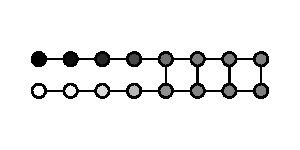
\includegraphics[scale=0.8]{plots/guattery-global}}
    \caption{Global partition from first nontrivial eigenvector of the Laplacian}
\end{figure}



Let $G$ be a graph with combinatorial Laplacian $L_G$, and let
$L_G^+$ denote its pseudoinverse. The pseudoinverse of the Laplacian is closely
related to random walks on the graph.  In particular, 
$L_{G}^{+}$ defines a proximity measure on the graph with the
following properties:
\begin{description}
  \item[Symmetry]
    $L_G^{+}(u,v) = L_G^{+}(v,u)$;
 \item[Diagonal maximality]
    $L_G^{+}(u,u) > L_G^{+} (u,v)$ whenever $u \neq v$;
  \item[Triangle inequality for proximities]
    If $u$ and $v$ are in the same connected component, then
    $L_G^{+} (u,v) + L_G^{+} (u,w) - L_G^{+} (v,w) \leq L_G^{+} (u,u)$, with strict inequality
    holding when $v = w$ and $u \neq v$;
  \item[Metric representability]
   $L_G^{+} (u,u) + L_G^{+} (v,v) - L_G^{+} (u,v) - L_G^{+} (v,u)$
    defines a metric on every connected component of $V_G$;  this is commonly called
    \emph{resistance distance} on $G$.
 \item[Transit property]
    if $G$ contains a path from $u$ to $v$, and each path from $u$ to
    $v$ includes $w$, distinct from $u$ and $v$, then $L_G^{+}(u,w) >
    L_G^{+}(u,v)$.
\end{description}
These properties follow from Chebotarev and Shamis' topological
representation of of the combinatorial Laplacian
\cite{chebotarev1998proximity}.  A full discusion of this
representation is beyond the scope of the present treatment, but for
unweighted, connected graphs, the authors show that if $|V_G| = n$,
then
\[
  L_G^{+}(u,v) = \frac{|\mathcal{F}_{n-2}^{uv}| - \frac{1}{n}
    \sum_{w} |\mathcal{F}_{n-2}^{uw}|}{|\mathcal{F}_{n-1}|},
\]
where $\mathcal{F}_k$ and $\mathcal{F}_k^{uv}$ are sets of subgraphs
of $G$; the set $\mathcal{F}_{k}$ comprises all rooted spanning forests
with $k$ edges, and $\mathcal{F}_{k}^{uv}$ comprises all rooted spanning
spanning forests with $k$ edges such that $u$ is a root, and $v$
belongs to the same tree as $u$.  Chandra et al.\ show that the
quantity $L_G^{+} (u,u) + L_G^{+} (v,v) - L_G^{+} (u,v) - L_G^{+} (v,u)$ is
proportional to the length of time before a random walker started at
node $u$ reaches node $v$ whenever $u$ and $v$ are in the same
connected component \cite{chandra1989electrical}.  It is likely that $L_G^{+}(u,v)$ has a
probabalistic interpretaiton in terms of random walks on the graph,
but we do not know of any such interpretation.

Given a cutoff value, $K$, we can define a local partition around node
$u$ via $P_K(u) = \{ v : L_G^{+}(u,v) > K \}$.  Note that if $v$ is in
$P_K(u)$, then $u$ is in $P_K(v)$.  In light of the disconnection
condition, if the graph is disconnected, then there exists a $K$ such
that $u$ and $v$ are in the same connected component iff
$v \in P_K(u)$.  We call this partitioning ``local spectral
clustering.''

\begin{figure}
    \centering
    \makebox{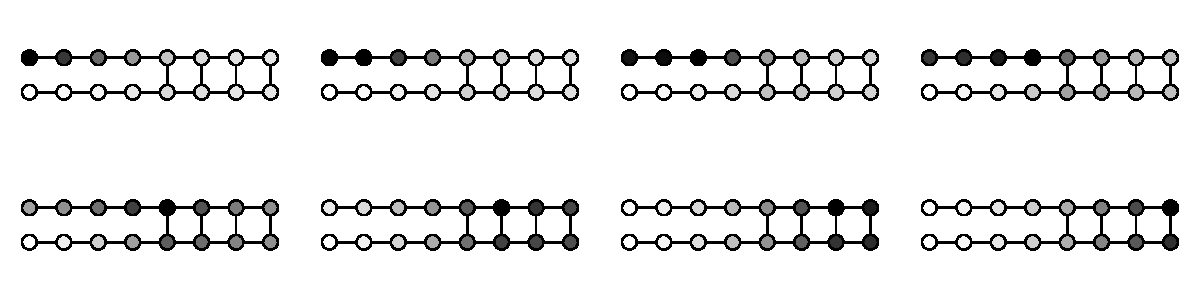
\includegraphics[scale=0.6]{plots/guattery-local}}
    \caption{Local partitions from the pseudoinverse of the Laplacian}
\end{figure}
\begin{figure}
    \centering
    \makebox{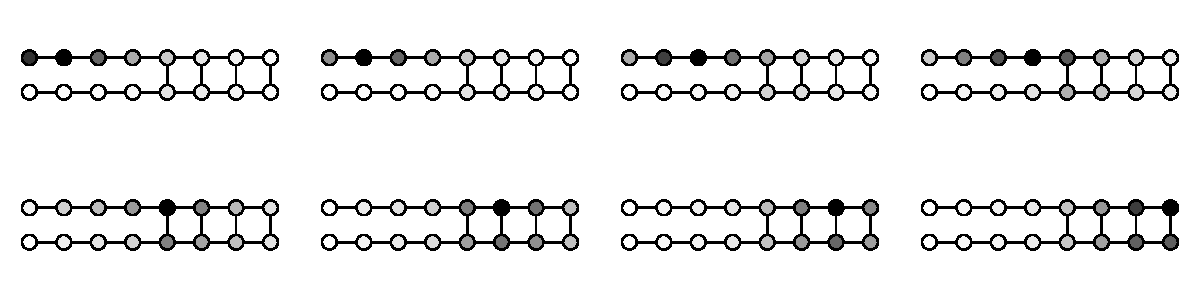
\includegraphics[scale=0.6]{plots/guattery-pagerank}}
    \caption{Local partitions from PageRank}
\end{figure}

[Add Guattery example here, showing benefits of local spectral.]


\subsection{Diffusion clustering}

In practrice, the pseudoinverse of the Laplacian is seldom (if ever)
use to partition the nodes of a graph.  The more common alternatives
to spectral clustering involve random walks or diffusions on the
graph.  These approaches assign positive and negative to the nodes,
and then let the distribution of charge evolve according to dynamics
derived fromt the graph structure (for example, Anderson et al.'s local
PageRank takes this approach \cite{andersen2006local}).
Three canonical evolution dynamics are the following
\begin{description}
  \item[heat kernel]
    charge evolves according to the dynamics of the heat equation
    $\frac{\partial H_t}{\partial t} = - L_G H_t$;
  \item[PageRank]
    charge at a node evolves by either teleporting to a random node or moving
    to a neighber of the current node;
  \item[lazy random walk]
    charge either stays at the current node or moves to a neighbor.
\end{description}
Mahoney and Orecchia showed that the above dynamics arrise
as solutions to semi-definite programs of the form
\[
\begin{aligned}
  & \underset{X}{\text{minimize}}
  & & \mathrm{tr}(L_G X) + F(X) \\
  & \text{subject to}
  & & X \succeq 0, \\
  & & & \mathrm{tr}(X) = 1, \\
  & & & \mathrm{tr}(X J) = 0,
\end{aligned}
\]
where $J = 1_{V_G} 1_{V_G}'$ and $F$ is a penalty function
\cite{mahoney2010implementing}.  Notably, when $F = 0$, the solution
to the above SDP is $u u'$, where $u$ is the smallest nontrivial
eigenvector of $L_G$.  Thus, in some sense, the heat kernel, PageRank,
and lazy random walk dynamics can be seen as ``regularized'' versions
of spectral clustering, where the function $F$ is acting as a penalty
function, analogous to the penalty in ridge regression or LASSO.

In the sequal, we extend Mahoney and Orecchia's
result, showing that solutions to the regularized SDP can be
interpreted as regularized estimates of the pseudoinverse of the
Laplacian.  Specifically, we set up a sampling model, whereby the
Laplacian is interpreted as an observation from a random process.  We
posit the existence of a ``population Laplacian'' driving the random
process.  We then define an estimation problem: finding the inverse of
the population Laplacian.  It turns out that the solution to the
regularized SDP arrises as the maximium a posteriori probability (MAP)
estimate of the inverse of the population Laplacian.  The role of the
penalty funciton, $F$, is to encode prior assumptions about the
population Laplacian.

Our approach is reminiscent of the Bayesian interpretation of
regularized linear regression.  In linear regression, an $L^2$ penalty
corresponds to a Gaussian prior on the coefficent vector, and the
solution to the regularized regression problem is the maximium a
posterior (MAP) estimator.  In the same setting, $L^1$ regularization
corresponds to a Laplace prior on the coefficent vector.


\section{A statistical framework for regularized graph estimation}

Here we lay out a simple Bayesian framework for estimating a graph
Laplacian, which allows for regularization by incorporating prior
information.  We suppose that the observed graph Laplacian, $L$, is a
random object whose distrubution depends on a true ``population''
Laplacian, $\mathcal{L}$.  This induces a conditional density for $L$,
denoted $p(L \mid \mathcal{L})$.  Next, we assume prior information
about the population Laplacian in the form of a prior density,
$p(\mathcal{L})$.  Given the observed Laplacian, we estimate the
population Laplacian by maximizing its posterior density,
$p(\mathcal{L} \mid L)$.


\subsection{Analogy with regularized linear regression}

It will be helpful to keep in mind the Bayesian
interpretation of regularized linear regression.  In that context, we
observe $n$ predictor-response pairs in $\reals^p \times \reals$,
denoted $(x_1, y_1), \dotsc, (x_n, y_n)$; the goal is to find a vector
$\beta$ such that $\beta' x_i \approx y_i$.  Typically, we choose
$\beta$ by minimizing the residual sum of squares,
$\RSS(\beta) = \sum_i \| y_i - \beta' x_i \|_2^2$, or a
penalized version of it.  For ridge regression, we minimize
$\RSS(\beta) + \lambda \|\beta\|_2^2$; for LASSO regression, we minimize
$\RSS(\beta) + \lambda \|\beta\|_1$.  The additional terms in the
optimization criteria ($\lambda \|\beta\|_2^2$ and $\lambda
\|\beta\|_1$) are called penalty functions.

Adding a penalty function to the optimization criterion can be
interpreted as incorporating prior information about $\beta$.  We
model $y_1, \dotsc, y_n$ as independent random observations with
distributions dependent on $\beta$.  Specifically, we suppose $y_i$ is
a Gaussian random variable with mean $\beta' x_i$ and known variance
$\sigma^2$.  This induces a conditional density for the vector
$y = (y_1, \dotsc, y_n)$:
\begin{equation}\label{E:regression-density}
  p(y \mid \beta)
    \propto
     \exp\{ -\tfrac{1}{2 \sigma^2} \RSS(\beta) \},
\end{equation}
where the constant of proportionality depends only on $y$ and $\sigma$.
Next, we assume that $\beta$ itself is random, drawn from a
distribution with density $p(\beta)$.  This distribution is called a
prior, since it encodes prior knowledge about $\beta$.  Without loss
of generality, the prior density can be assumed to take the form
\begin{equation}\label{E:regression-prior}
  p(\beta) \propto \exp\{ -\tfrac{1}{2} F(\beta) \}.
\end{equation}
Since the two random variables are dependent, upon observing $y$, we
have information about $\beta$.  This information is incoded in the
posterior density, $p(\beta \mid y)$, computed via
Bayes' rule as
\begin{equation}\label{E:regression-posterior}
  p(\beta \mid y)
    \propto p(y \mid \beta) \, p(\beta)
    \propto \exp\{ -\tfrac{1}{2 \sigma^2} \RSS(\beta) - \tfrac{1}{2} F(\beta) \}.
\end{equation}
The maximum a posterior probablility (MAP) estimate of $\beta$ is the
value that maximizes $p(\beta \mid y)$.  Equivalently, $\beta$
minimizes $\log p(\beta \mid y)$.  We can recover the solution to
Ridge or LASSO regression by setting
$F(\beta) = \tfrac{\lambda}{\sigma^2} \| \beta \|_2^2$ or
$F(\beta) = \tfrac{\lambda}{\sigma^2} \| \beta \|_1$.  Thus, Ridge
regression can be interpeted as imposing a Gaussian prior on $\beta$,
and LASSO regression can be interpreted as imposing a
double-exponential prior on $\beta$.


\subsection{Bayesian inference for the population Laplacian}

Suppose $L$ is the normalized Laplacian of a connected graph with $n$
nodes.  Take $L$ to be a random object with expectation~$\mathcal{L}$,
where $\mathcal{L}$ is another normalized graph Laplacian.  We refer to $\mathcal{L}$ as the
``population'' graph Laplacian, and we refer to $L$ as the ``sample''
graph Laplacian.  In general, $\mathcal{L}$ can be distinct from $L$,
but we require that the nodes in the population and sample graphs have
the same degrees, given by the vector $d = \big(d(1), \dotsc,
d(n)\big)$. Let $D = \diag\big(d(1), \dotsc, d(n)\big)$ and let
$\mathcal{X} = \{ X : X \succeq 0, \, X D^{1/2} 1 = 0, \, \rank(X) = n - 1 \}$.  The
population and sample Laplacians are both members of $\mathcal{X}$.


To apply the Bayesian formalism, we need to fully specify the
conditional density of $L$ given $\mathcal{L}$.  A convenient choice
is to take $L$ to be a scaled Wishart matrix with expectation
$\mathcal{L}$.  Specifically, let $m \geq n - 1$ be a scale parameter
and suppose $L$ is distributed as a
$\tfrac{1}{m} \mathrm{Wishart}(\mathcal{L}, m)$ random variable.
Thus, $\E[L \mid \mathcal{L}] = \mathcal{L}$ and $L$ has conditional density
\begin{equation}\label{E:density}
  p(L \mid \mathcal{L})
    \propto
      \frac{\exp\{ -\frac{m}{2} \Tr(L \mathcal{L}^+)\}}
           {|\mathcal{L}|^{m/2}},
\end{equation}
where $|\cdot|$ denotes pseudodeterminant (product of nonzero
eigenvalues).  The constant of proportionality depends only on $L$,
$d$, $m$, and $n$, and the density is supported on $\mathcal{X}$.
Eq.~\eqref{E:density} is analogous to Eq.~\eqref{E:regression-density}
in the linear regression context.

Now suppose we have know that $\mathcal{L}$, is a random object drawn
from a prior density $p(\mathcal{L})$.
Without loss of generality,
\begin{equation}\label{E:prior}
  p(\mathcal{L}) \propto \exp\{ -\tfrac{1}{2} F(\mathcal{L}^+) \},
\end{equation}
for some function $F$, supported on a subset
$\mathcal{S} \subseteq \mathcal{X}$.  (The space $\mathcal{X}$ is
closed under inversion, so if $\mathcal{L}^{+} \in \mathcal{S}$, then
$\mathcal{L} \in \mathcal{X}$.)
Eq.~\eqref{E:prior} is analogous to Eq.~\eqref{E:regression-prior}.

Upon observing $L$, the posterior distribution for $\mathcal{L}$ is
\begin{equation}\label{E:posterior}
  p(\mathcal{L} \mid L)
    \propto p(L \mid \mathcal{L}) \, p (\mathcal{L})
    \propto \exp\{ -\tfrac{m}{2} \Tr(L \mathcal{L}^+)
                   + \tfrac{m}{2} \log |\mathcal{L}^+|
                   - \tfrac{1}{2} F(\mathcal{L^+}) \},
\end{equation}
with support determined by $\mathcal{S}$.  Eq.~\eqref{E:posterior} is
analogous to Eq.~\eqref{E:regression-posterior}.  The MAP estimator of
$\mathcal{L}^+$ is the solution to the program
\[
\begin{aligned}
  & \underset{X}{\text{minimize}}
  & & \Tr(L X) + \tfrac{1}{m} F(X) - \log |X| \\
  & \text{subject to}
  & & X \in \mathcal{S}.
\end{aligned}
\]
Note the similarity with Mahoney and Orecchia's relaxed SDP.
In particular, if
\(
  \mathcal{S} = \{ X : \Tr(X) = 1 \} \cap \mathcal{X},
\)
then the two programs are identical except for the factor of
$\log |X|$ in the optimization criterion.  More generally, if
$\mathcal{S} = \{ X : \Tr(X) = \tau^{-1} \} \cap \mathcal{X}$,
then the MAP estimator of
$[\Tr(\mathcal{L}^{+})]^{-1} \mathcal{L}^{+} = \tau \mathcal{L}^+$
is the solution to the program
\[
\begin{aligned}
  & \underset{X}{\text{minimize}}
  & & \Tr(L X) + \tfrac{\tau}{m} F(\tau^{-1} X) - \tau \log |X| \\
  & \text{subject to}
  & & X \succeq 0 \\
  & & & X D^{1/2} 1 = 0 \\
  & & & \Tr(X) = 1
\end{aligned}
\]




\clearpage

Let $G$ be a graph with vertex set $V = \{ 1, 2, \dotsc, n \}$, edge
set $E = V \times V$ equipped with the equivalence relation
$(u,v) = (v,u)$.  Let $\omega$ be an edge weight function, and let
$\mathcal{L}$ be the corresponding Laplacian.  Assume without loss of
generality that $\sum_{(u,v) \in E} \omega(u,v) = 1$.  We interpet
$\omega$ and $\mathcal{L}$ as unobserved ``population'' quantities,
referring to $\omega(u,v)$ as the population weight of edge $(u,v)$,
and referring to $\mathcal{L}$ as the population Laplacian.

Suppose we sample $m$ edges from the $E$, randomly chosen
according to the population weight function.  That is, we see edges
$(u_1, v_1), (u_2, v_2),  \dotsc, (u_m, v_m)$, where the edges are
all drawn independently and identically such that the probability of
seeing edge $(u,v)$ is
\[
  \prob_\omega\{ (u_1, v_1) = (u,v) \} = \omega(u,v).
\]
Notably, we will likely see duplicate edges, and not every edge with a
positive weight will get sampled.

We construct a weight function from the sampled edges, called the
sample weight function, $w$, defined such that
\[
  w(u,v) = \frac{1}{m} \sum_{i=1}^{m} 1\{ (u_i, v_i) = (u,v) \}.
\]
In turn, we construct a sample Laplacian, $L$, defined such that
\[
  L(u,v)
    =
    \begin{cases}
      \sum_{w \neq u} w(u,w) &\text{when $u = v$,} \\
      -w(u,v) &\text{otherwise.}
    \end{cases}
\]
Note that $\E_\omega[w(u,v)] = \omega(u,v)$ and $\E_\omega L =
\mathcal{L}$, where $\E_\omega$ denotes expecation with respect to
probability law $\prob_\omega$.

Our goal is to estimate the pseudoinverse of the population Laplacian,
$\mathcal{L}^{+}$, using only the sampled edges.  The obvious estimate
is $L^{+}$, the pseudoinverse of the sample Laplacian.  We can often
do better when we have prior information about $\mathcal{L}$.

The form of our prior information comes in the form of a prior distribution
for $\mathcal{L}$.  That is, we think of $\mathcal{L}$ as a random
object, drawn from some prior distribution.  If we think that
$\mathcal{L}$ comes from an ``expander-like'' graph, then our prior
distribution for $\mathcal{L}$ will put most of its weight on
expander-like graphs.  Correspondingly, if we think that $\mathcal{L}$
comes from a graph that can be embedded in a low-dimensional space,
then our prior distribution for $\mathcal{L}$ will put most if its
weight on such graphs.

Let $p(\mathcal{L})$ denote our prior for $\mathcal{L}$, assumed to be
an arbitrary density over the space of graph Laplacians.  Likewise, let
$p(L \mid \mathcal{L})$ denote the density for the
distribution of $L$, conditional on $\mathcal{L}$.  Using Bayes' rule,
the posterior destribution for $\mathcal{L}$ after having observed $L$
is proportional to $p(L \mid \mathcal{L}) \, p(\mathcal{L})$.
Conceptually, Bayes' rule gives us a straightforward to
incorporate prior information into our estimate of $\mathcal{L}^+$.
We can get an estimate of $\mathcal{L}^{+}$ be maximizing the
posterior distribution for $\mathcal{L}$.

\subsection{Approximate likelihood for the sample Laplacian}

The conditional density $p(L \mid \mathcal{L})$ is defined completely
by the edge sampling scheme we laid out above.   However, the exact
expression for $p(L \mid \mathcal{L})$ involves an intractible
combinatorial sum.  We appeal to a crude approximation for the conditional
density $p(L \mid \mathcal{L})$.  The approximaton works as follows:
\begin{enumerate}
\item For $i = 1, \dotsc, m$, define $x_i \in \reals^n$ such that
  \[
    x_i(u)
      =
      \begin{cases}
        +s_i &\text{when $u = u_i$,} \\
        -s_i &\text{when $u = v_i$,} \\
        0 &\text{otherwise,}
      \end{cases}
  \]
  where $s_i \in \{ -1, +1 \}$ is chosen arbitrarily.
\item Note that $L = \sum_{i=1}^m x_i x_i'$.
\item Take $s_i$ to be random, equal to $+1$ or $-1$ with probability
  $\tfrac{1}{2}$.  Approximate the distribution of $x_i$ by the
  distribution of a multivariate normal random variable, $\tilde x_i$,
  such that $x_i$ and $\tilde x_i$ have the same first and second
  moments.
\item Approximate the distribution of $L$ by the distribution of $\tilde L$, where
  \(
    \tilde L = \sum_{i=1}^m \tilde x_i \tilde x_i'.
  \)
\end{enumerate}

\noindent
The next two lemmas derive the distribution of $\tilde x_i$ and
$\tilde L$ in terms of $\mathcal{L}$, allowing us to get an
approximation for $p(L \mid \mathcal{L})$.

\begin{lemma}
  With $x_i$ and $\tilde x_i$ defined as above,
  \[
    \E_\omega[ x_i ] = \E_\omega[ \tilde x_i ] = 0,
  \]
  and
  \[
    \E_\omega[ x_i x_i' ] = \E_\omega [ \tilde x_i \tilde x_i' ] = \mathcal{L}.
  \]
\end{lemma}
\begin{proof}
  The random variable $\tilde x_i$ is defined to have the same first
  and second moments as $x_i$.
  The first momemnt vanishes since $s_i \overset{d}{=} -s_i$ implies
  that $x_i \overset{d}{=} -x_i$.  For the second moments, note that
  when $u \neq v$, 
  \[
    \E_\omega[x_i(u) \, x_i(v)]
      = -s_i^2 \, \prob_\omega\{ (u_i,v_i) = (u,v) \}  = -\omega(u,v)
      = \mathcal{L}(u,v).
  \]
  Likewise,
  \[
    \E_\omega[\{x_i(u)\}^2]
      = \sum_{v} \prob_\omega\{ (u_i,v_i) = (u,v) \}
      = \sum_{v} \omega(u,v)
      = \mathcal{L}(u,u).
  \]
\end{proof}

\begin{lemma}\label{L:approx-wishart}
  The random matrix $\tilde L$ is distrubted as a Wishart matrix with
  shape $\mathcal{L}$ and scale $m$.  This distribution, denoted
  $\mathcal{W}(\mathcal{L}, m)$ is supported on the set of
  positive-semidefinite matrices with the same nullspace as $\mathcal{L}$.  When
  $m \geq \rank(\mathcal{L})$, the distribution has a denisty on this space
  given by
  \begin{equation}\label{E:wishart-density}
    f_\mathcal{W}( \tilde L \mid \mathcal{L}, m)
      \propto
      \frac{|\tilde L|^{(m - \rank(\mathcal{L}) - 1)/2}
        \exp\{-\tfrac{1}{2} \Tr(\tilde L \mathcal{L}^+) \}}
        {|\mathcal{L}|^{m/2}}
  \end{equation}
  where the constant of proportionality depends only on $m$ and $\rank(\mathcal{L})$,
  and where $|\cdot|$ denotes pseudodeterminant (product of nonzero
  eigenvalues).
\end{lemma}
\begin{proof}
  Since $\tilde L$ is a sum of $m$ outer products of multivariate
  $\mathrm{Normal}(0, \mathcal{L})$, it is Wishart distributed
  (by definition).
  Suppose $\rank(\mathcal{L}) = r$ and
  $U \in \reals^{n \times r}$ is a matrix whose columns are the
    eigenvectors of $\mathcal{L}$.  Note that
    $U' \tilde x_i \overset{d}{=} \mathrm{Normal}(0, U' \mathcal{L} U)$,
    and that $U' \mathcal{L} U$ has full rank.  Thus,
    \(
      U' \tilde L U
    \)
    has a density over the space of $r \times r$ positive-semidefinite
    matrices whenever $m \geq r$.  The density of $U' \tilde L U$ is
    exactly equal to $f_\mathcal{W}(\tilde L \mid \mathcal{L}, m)$,
    defined above.
\end{proof}


\subsection{Approximate posterior inference}

Lemma~\ref{L:approx-wishart} gives us an approximation for
$p(L \mid \mathcal{L})$.  Namely, we can approximate
$p(L \mid \mathcal{L})$ by
$\tilde p(L \mid \mathcal{L}) = f_\mathcal{W}(L \mid \mathcal{L}, m)$,
where $f_\mathcal{W}$ is as defined in Eq.~\eqref{E:wishart-density}.
With a specification for the prior density $p(\mathcal{L})$, we can
get an approximation to the posterior denisty:
\[
  p(\mathcal{L} \mid L)
  \approx
  \tilde p(\mathcal{L} \mid L)
    \propto \tilde p(L \mid \mathcal{L}) \, p(\mathcal{L}).
\]
We can then estimate $\mathcal{L}$ by maximizing
$\tilde p(\mathcal{L} \mid L)$.

Suppose the prior takes the form
\[
  p(\mathcal{L}) \propto \exp\{ -\tfrac{1}{2} F(\mathcal{L^+}) \}
\]
for some function, $F$, supported on a subset, $\mathcal{S}$, of all
positive-semidefinite matrices.  An approximation to the
maximum a posteriori probability estimate of $\mathcal{L}$ maximizes
$\tilde p(\mathcal{L} \mid L)$.  Suppose that the
matrices in $\mathcal{S}$ have the same rank, which is less than or
equal to $m$.
Up to a constant, twice the negative logarithm of the optimization criterion is
\begin{align*}
  -2 \log \tilde p(\mathcal{L} \mid L)
   &= - 2 \log \tilde p(L \mid \mathcal{L}) - 2 \log p(\mathcal{L}) \\
   &= \Tr(L \mathcal{L}^+) + F(\mathcal{L^+}) - m \log | \mathcal{L}^+ |
\end{align*}
The approximate MAP for $\mathcal{L}^+$ is the solution to the program
\[
\begin{aligned}
  & \underset{X}{\text{minimize}}
  & & \Tr(L X) + F(X) - m \log |X| \\
  & \text{subject to}
  & & X^+ \in \mathcal{S}.
\end{aligned}
\]
Note the similarity with Mahoney and Orecchia's relaxed SDP.
In particular, if
\(
  \mathcal{S} = \{ \mathcal{L} : \mathcal{L} \succeq 0,
  \Tr(\mathcal{L} J) = 0, \Tr(\mathcal{L}^{+} J) = 1 \},
\)
then the two programs are identical except for the factor
$-m \log |X|$ in the optimization criterion.


\section{Prior specification}

To successfully leverage the results in the preceding section, we need
to choose densities $p(\mathcal{L})$ that encode our prior beliefs in
particular application regimes.  In this section, we present three
parametric forms for the prior that allow us to interpolate between
``expander-like'' graphs and ``low-dimensional'' graphs.

We encode information about the
``low-dimensionality'' or ``expanderness'' of a network through its
spectrum.  For a network to be expander-like, we expect the gaps
between consecutive eigenvalues of the Laplacian to be small.  For a
network to be low-dimensional, we expect the smallest non-trivial
eigenvalues to be well-separated from the rest of the spectrum.

\begin{figure}
    \centering
    \makebox{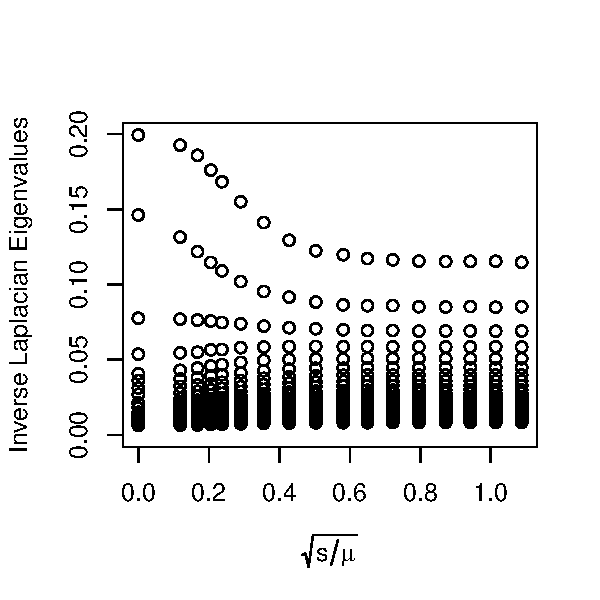
\includegraphics[scale=0.6]{plots/interpolate}}
    \caption{Interpolating from a low-dimensional graph to an expander}
\end{figure}



\subsection{Support sets}

The support sets of the priors are subsets of the
positive-semidefinite matrices.  Take $\mathcal{S}$ to be a typical
support set.  Firstly, since every combinatorial Laplacian
$\mathcal{L}$ satisfies $\mathcal{L} 1 = 0$, we will generally require
this property of all matrices in $\mathcal{S}$.  Secondly, since the
scale of the Laplacian cannot be identified in our samply scheme
(i.e., the distribution of $L$ remains unchanged if $\mathcal{L}$ is
replaced by $c \cdot \mathcal{L}$ for any positive constant $c$), we
fix a scale for the matrices in $\mathcal{S}$.  A convenient way of
fixing the scale is to specify that $\Tr(\mathcal{L}^+) = 1$ for
all $\mathcal{L}$ in $\mathcal{S}$.  Finally to avoid undue technical
complications, we require that all matrices in $\mathcal{S}$ have rank
$n-1$.



\subsection{Densities}

The priors we specify only depend on the eigenvalues of the Laplacian.
Equivalently, they depend on the eigenvalues of the pseudoinverse of
the Laplacian.  If $\mathcal{L}^+ = U \Lambda U'$ is the spectral
decomposition of the pseudoinverse of Laplacian $\mathcal{L}$, where
$U \in \reals^{n \times n -1}$ and
$\Lambda = \diag\big(\lambda(1), \dotsc, \lambda({n-1})\big)$, then the prior
weight on $\mathcal{L}$ only depends on $\Lambda$.  The implication is
that $U$ is uniformly distributed over the space of orthogonal
matrices satisfying $(n-1) U U' \in \mathcal{S}$, where $\mathcal{S}$ is the
support set of the prior.  This follows since $U'1 = 0$ and $\Tr([(n-1) U U']^+) =
\Tr((n-1)^{-1} U U') = 1$.

The priors below all take the form $p(\mathcal{L}) \propto
\exp\{-\tfrac{1}{2} F(\mathcal{L}^{+})\}$, where $F(\mathcal{L}^{+})$
depends only on $\Lambda = \diag(\lambda_1, \dotsc, \lambda_{n-1})$, the nonzero
eigenvalues of $\mathcal{L}^{+}$.  They all depend on a
meta-parameter, $\eta$:

\begin{description}
  \item[Generalized entropy]
    \[
      F_H(\mathcal{L}^+) = \tfrac{1}{\eta}[ \Tr( \Lambda \log \Lambda)
      - \Tr(\Lambda)];
    \]
  \item[Log-determinant]
    \[
      F_D(\mathcal{L}^{+}) = - \tfrac{1}{\eta} \log |\Lambda|;
    \]
  \item[Standard $k$-norm]
    \[
      F_k(\mathcal{L}^+)
        = \frac{1}{k \, \eta} \Tr(\Lambda^k).
  \]
\end{description}
 
For the log-determinant prior, we have
\[
  p(\mathcal{L})
    \propto \prod_{v=1}^{n-1} \lambda(v)^{1/2 \eta},
\]
i.e. the nonzero eigenvalues of $\mathcal{L}^{+}$ are
Dirichlet-distributed over the simplex with parameters $\alpha(1) =
\alpha(2) = \dotsb = \alpha(n-1) = 1 + \tfrac{1}{2\eta}$.  The other
priors do not correspond to standard parametric forms.

For all three parametric forms, by varying $\eta$ we can put more or
less prior weight on expanders or low-dimensional graphs.

\begin{figure}
    \centering
    \makebox{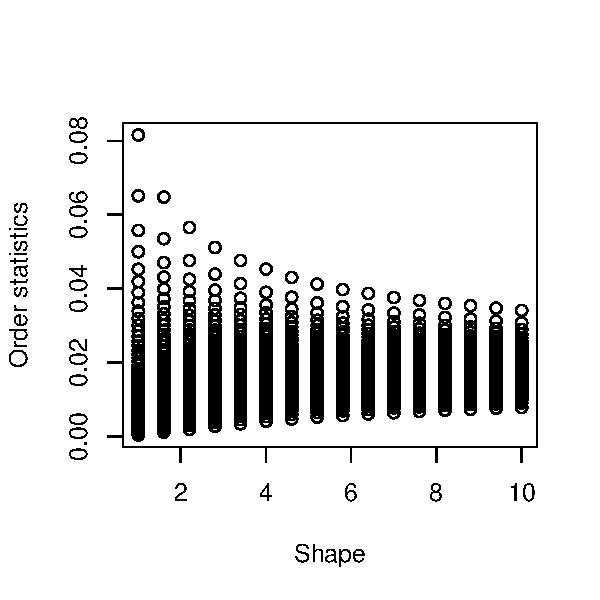
\includegraphics[scale=0.6]{plots/dirichlet}}
    \caption{Dirichlet distriubtion order statistics}
\end{figure}

\section{Empirical evaluation}

\section{Concluding remarks}

\bibliographystyle{plain}
\bibliography{refs}

\end{document}
